\section{Analyse et Conception}

Comme tout projet de développement, il faut commencer par une phase d'analyse et de conception. Le projet Open Data Event a comme particularité d'avoir déjà eu plusieurs versions avant que je ne commence à travailler dessus. C'est pourquoi la partie d'analyse des versions précédentes était très importante, comme vous pourrez le lire par la suite.

\subsection{Mise en place de mon environnement de travail}

Il a été mis à ma disposition un \textbf{iMac} 21" avec un second écran de la même taille. J'ai donc pu découvrir l'environnement de développement offert par \textbf{OS X}. Globalement, la connaissance de l'environnement \textbf{Linux} m'aura aidé tout au long de l'utilisation d'OS X.

Après m'être créé un compte administrateur sur l'ordinateur fourni, j'ai pu installer tous les logiciels nécessaires à la réalisation du projet. Pour des raisons personnelles, j'ai choisi d'utiliser les outils suivants:

\begin{itemize}
    \item \textbf{iTerm} (Version 2.0.0)
    \item \textbf{Sublime Text 2} (Version 2.0.2)
    \item \textbf{Google Chrome} (Version 43)
    \item \textbf{Wireshark} (Version 1.12.5)
    \item \textbf{Apple Calendar} (Version 7.0)
    \item \textbf{PDFLatex} (Version 3.14)
\end{itemize}

Pour l'utilisation de serveurs SabreDAV, Baïkal, ElasticSearch et d'autres, j'ai installé une machine virtuelle avec \textbf{Vagrant}.

\textbf{LiberTIC} étant une association militant pour les licences libres, il était évident que la majorité de mon travail (qu'il s'agisse de développement ou de comptes-rendus) soit mis lui aussi sous licence libre. Ainsi, il est possible de retrouver mon travail sur \textbf{GitHub} à l'adresse suivante: \url{https://github.com/LiberTIC/ODEV2}.

En plus de mon environnement local, j'ai pu accéder à un serveur de préproduction hébergé par OVH.

\subsection{Mise à niveau préliminaire}

Dès le début de mon stage, il a été défini que le projet allait se construire sur des technologies que je ne connaissais pas et/ou ne maîtrisais pas. C'est pourquoi il a été convenu que la première semaine de mon stage serait consacrée à une mise à niveau pour différentes technologies.

Premièrement, j'ai suivi un récapitulatif des commandes \textbf{Git} \rf{gitimmersion} puis lu un article sur les bonnes pratiques de l'utilisation de Git et de ses branches \rf{successfulgit}.

Ensuite, j'ai lu plusieurs articles sur les bonnes pratiques du développement \textbf{PHP} \rf{bestpracticephp} \rf{stupidvssolid}.

Enfin, j'ai lu et appliqué la totalité du \textbf{Symfony Book} \rf{symfonybook}. Il s'agit du document de référence dans l'apprentissage du Framework. Ce document est mis à jour très régulièrement et permet d'obtenir une grande partie des informations nécessaires pour se lancer dans le développement d'une application Symfony 2.

\subsection{Analyse des besoins}

\subsubsection*{Service en ligne}

Une volonté de la part de LiberTIC était de faire d'ODE un service disponible en ligne. 
Sachant que j'ai effectué mon stage en partenariat chez Les Polypodes et que Symfony 2 est la Stack la mieux maîtrisée par l'équipe, c'était le choix le plus logique pour pouvoir être accompagné par toute l'équipe en cas de besoin.

Symfony 2 est un framework PHP proposant un grand nombre de composants facilitant et accélérant le travail du développeur PHP.

\subsubsection*{CMS adapté}

Un des besoins les plus importants de la version 2 était de pouvoir proposer un Content Manager System accessible, dont même une personne ne connaissant rien à l'informatique pourrait ajouter du contenu.

\subsubsection*{API REST}

Sachant qu'une partie importante de l'Open Data consiste en la réutilisation des données, il parut important de proposer une API REST pour récupérer les événements.

\subsubsection*{Compatibilité}

Un des souhaits de la part d'ODE était de rendre compatible l'application avec d'autres clients calendriers. J'en parlerai plus tard avec l'introduction de CalDAV.

\subsection{Conception et première réunion}

Une semaine après le début de mon stage, j'ai pu rencontrer deux personnes de l'association durant une réunion où nous avons discuté ensemble du périmètre du projet ainsi que ce que je proposais pour l'architecture.

\subsubsection*{Diagramme de cas d'utilisation}

Suite à la conception, j'ai fait un diagramme de cas d'utilisation de l'application. Il est possible de le retrouver dans les Annexes à la dernière page de ce rapport.

\subsubsection*{CalDAV et WebDAV}

Dès la première réunion, il était clair qu'il fallait se baser sur un protocole déjà en place, pour ne pas `` réinventer la roue ''. Le seul protocole actuellement en place répondant à nos besoins est \textbf{CalDAV}. Il s'agit d'une extension du protocole WebDAV, lui même une extension du protocole HTTP (plus d'informations en Annexe 1). 

CalDAV définit la gestion des calendriers au sein d'un serveur. Il décrit aussi la façon dont les serveurs CalDAV doivent gérer les événements et les utilisateurs.

CalDAV est défini par la RFC 4791\rf{RFC4791} datant de 2007. Il existe plusieurs implémentations de cette RFC. La première, historiquement parlant, est CalendarServer, en python.

\subsubsection*{Ontologie}

Pour s'adapter au mieux au ``Web sémantique'', nous avons décidé qu'il était important de se documenter sur les ontologies déjà effectué sur l'événementiel. Nous avons donc étudié la proposition de Schema.org (\url{https://schema.org/Event}). Le resultat de cette recherche est disponible sous forme de tableau dans l'annexe 2.

\subsubsection*{oEmbed}

Durant la réunion, nous avons discuté de la façon dont ODE devrait gérer l'ajout de médias à un événement. Après s'être mis d'accord sur le fait que gérer l'upload d'images, de vidéos ou autres, ne serait pas intéressant, M. Ségalou a évoqué l'utilisation d'oEmbed (\url{http://www.oembed.com/}).

oEmbed est un format permettant d'obtenir des informations relatives à un média. Globalement, il suffit de fournir une URL appartenant à un service compatible oEmbed (Youtube, Flickr, Vimeo, DailyMotion, SoundCloud, etc.) (Figure 2). Ensuite, grâce à l'URL, il sera possible de récupérer des informations le concernant (Figure 3). Pour enfin l'afficher directement sur le site (Figure 4).

\newpage

\begin{figure}[H]
\begin{center}
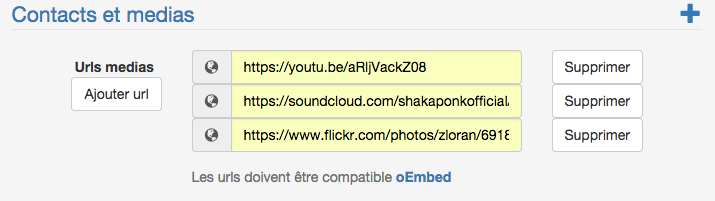
\includegraphics[height=30mm]{ajout_url_media.png}
\end{center}
\caption{Partie du formulaire pour ajouter des URL de médias}
\end{figure}


\begin{figure}[H]
\begin{lstlisting}[frame=single]
{
    "title": "Shaka Ponk - Wanna Get Free", 
    "width": 480, 
    "height": 270, 
    "thumbnail_height": 360, 
    "html": "\u003ciframe width=\"480\" height=\"270\" src=\"https:\/\/
www.youtube.com\/embed\/aRljVackZ08?feature=oembed\" frameborder=\"0\" 
allowfullscreen\u003e\u003c\/iframe\u003e", 
    "thumbnail_width": 480, 
    "author_url": "http:\/\/www.youtube.com\/user\/ShakaPonkVEVO", 
    "provider_name": "YouTube", 
    "version": "1.0", 
    "type": "video", 
    "provider_url": "http:\/\/www.youtube.com\/", 
    "author_name": "ShakaPonkVEVO", 
    "thumbnail_url": "https:\/\/i.ytimg.com\/vi\/aRljVackZ08\/
hqdefault.jpg"
}
\end{lstlisting}
\caption{Données récupérées depuis YouTube grâce au format oEmbed}
\end{figure}

\begin{figure}[H]
\begin{center}
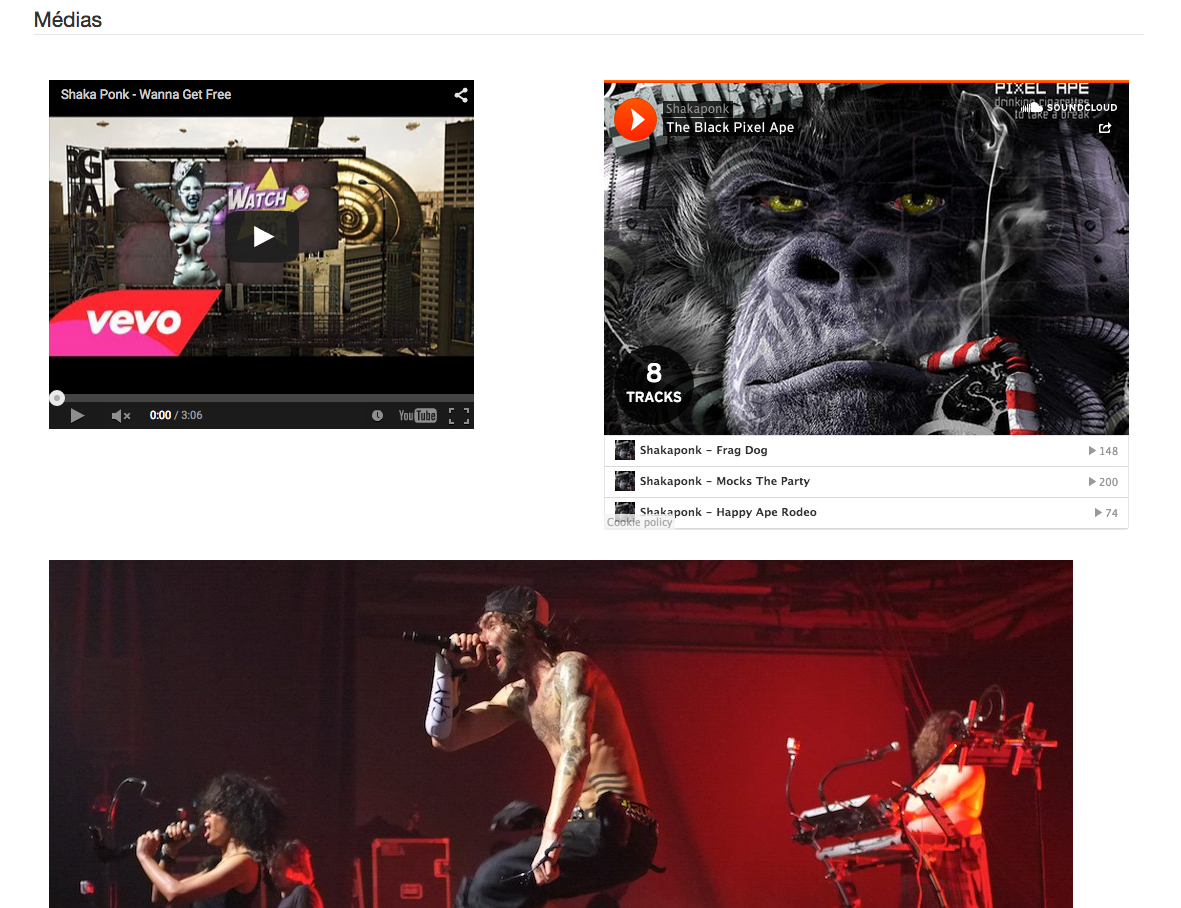
\includegraphics[height=70mm]{medias_embeded.png}
\end{center}
\caption{Médias affichés directement sur le site}
\end{figure}
